%%% LaTeX Template: Article/Thesis/etc. with colored headings and special fonts
%%%
%%% Source: http://www.howtotex.com/
% vim: set spell spelllang=es syntax=tex :

\documentclass[12pt]{article}
\usepackage{styles/apuntes-estilo}
\usepackage{fancyhdr,lastpage}
\usepackage{hyperref}
\usepackage[inline]{enumitem}
\usepackage{xurl}
\usepackage{nameref}
\usepackage{tabularx}

\usepackage{appendix}
\renewcommand{\appendixname}{Anexo}
\renewcommand{\appendixtocname}{Anexo}
\renewcommand{\appendixpagename}{Anexo}

\newcommand{\multiline}[2][c]{
      \begin{tabular}[#1]{@{}c@{}}#2\end{tabular}
      }

\def\maketitle{

\makeatletter{
    \color{blue} \centering \huge \sc
    \textbf{
        Trabajo práctico N° 8\\
        \large \vspace*{-8pt} \color{black}
        Arquitectura y organización de computadoras
        \vspace*{8pt}
    }\\
    \small Fecha de finalización: 7 de junio
    \par
}

\makeatother

\makeatletter
% vim: set spell spelllang=es syntax=tex :
 {\centering \small 
    Introducción a la computación\\
    Departamento de Ingeniería de Computadoras \\
    Facultad de Informática - Universidad Nacional del Comahue \\
    \vspace{20pt} }
\makeatother

\vspace{-2.5cm}
\mbox{\hspace{-1cm}\includegraphics[width=3cm,height=3cm]{logos/uncoma.pdf}\hspace{12cm}
    
\includegraphics[width=3cm,height=3cm]{logos/fai.pdf}}



}

% Custom headers and footers
\fancyhf{} % clear all header and footer fields
\fancypagestyle{plain}{\fancyhf{}}
\pagestyle{fancy}
\lhead{\footnotesize TP N° 8 - Arquitectura y organización de computadoras}
\rhead{\footnotesize \thepage\ }

\def\ti#1#2{\texttt{#1} & #2 \\ }

\begin{document}

\thispagestyle{empty}
\maketitle
\setlength{\parindent}{1pt}

\textbf{Objetivo:} Comprender la organización y el funcionamiento básico de
una computadora simple. Se involucran conocimientos de los componentes
hardware y sus interacciones para ejecutar instrucciones.

\textbf{Recursos bibliográfico:}

\vspace{-2\topsep}
\begin{itemize}

    \itemsep2pt \parskip0pt \parsep0pt

    \item \emph{Andrew S. Tanenbaum}. Organización de computadoras: un enfoque
        estructurado. Cuarta edición, editorial Pearson Educación, 2000. ISBN
        970-170-399-5.

\end{itemize}

\textbf{Lectura obligatoria:}

\vspace{-2\topsep}
\begin{itemize}

    \itemsep2pt \parskip0pt \parsep0pt

    \item Apuntes de cátedra. \emph{Capitulo 5: Arquitectura y Organización de
        Computadoras}, y \emph{Capitulo 7: El Software}. Disponible en:
        \url{https://egrosclaude.github.io/IC/IC-notes.pdf}

\end{itemize}

\section*{Modelo Computacional Binario Elemental (MCBE)}

Suponga la máquina \emph{MCBE} en su estado inicial con contenido de memoria
indicado en cada inciso (asuma por simplicidad que el resto de la memoria se
inicializa en cero). Describir el efecto de la ejecución de cada una de las
instrucciones del programa haciendo la traza de su ejecución. Luego explique
en lenguaje natural cual es el resultado de la ejecución del programa.

\begin{enumerate}

\item \begin{tabular}{| c | c |}
        \hline
        \textbf{Dirección}&\textbf{Contenido binario}\\
        \hline \hline
        0 & 01000111 \\
        \hline
        1 & 01111111 \\
        \hline
        2 & 10001000 \\
        \hline
        3 & 01100111 \\
        \hline
        4 & 11100010 \\
        \hline
        5 & 11011011 \\
        \hline
        6 & 00100000 \\
        \hline
        7 & 00000010 \\
        \hline
        8 & 11111111 \\
        \hline
        \hline
\end{tabular}

Ejemplo de Resolución:

{\tiny(Se utiliza el símbolo ``\textbf{-}'' para indicar que no se produjo
        ningún cambio)}

    { \scriptsize
    \begin{tabular}{|c|c||c|c||c|c|c|c|}
        \hline
        \multicolumn{2}{|c||}{\multiline{Búsqueda de la \\
        instrucción }} &
        \multicolumn{2}{|c||}{\multiline{Decodificación de la \\
        instrucción}} &
        \multicolumn{4}{|c|}{Ejecución de la instrucción}\\
        \hline
        PC & IR & Cod. Op. & Operando & Acumulador & Memoria &
        Salida & PC \\
        \hline
        00000000 & 01000111 & 010 & 00111 & 00000010 & - & - & 00000001 \\
        \hline
        00000001 & 01111111 & 011 & 11111 & - & - & 00000010 & 00000010 \\
        \hline
        00000010 & 10001000 & 100 & 01000 & 00000001 & - & - & 00000011 \\
        \hline
        00000011 & 01100111 & 011 & 00111 & - & (00000111)←00000001 & - & 00000100 \\
        \hline
        00000100 & 11100010 & 111 & 00010 & - & - & - & 00000101 \\
        \hline
        00000101 & 11011011 & 110 & 11011 & - & - & - & 00000000 \\
        \hline
        00000000 & 01000111 & 010 & 00111 & 00000001 & - & - & 00000001 \\
        \hline
        00000001 & 01111111 & 011 & 11111 & - & - & 00000001 & 00000010 \\
        \hline
        00000010 & 10001000 & 100 & 01000 & 00000000 & - & - & 00000011 \\
        \hline
        00000011 & 01100111 & 011 & 00111 & - & (00000111)←00000000 & - & 00000100 \\
        \hline
        00000100 & 11100010 & 111 & 00010 & - & - & - & 00000110 \\
        \hline
        00000110 & 00100000 & 001 & 00000 & - & - & - & - \\
        \hline
    \end{tabular}
    }

\textbf{Descripción en lenguaje natural:} El programa imprime 2 y 1, y luego
termina su ejecución.

\item \begin{tabular}{| c | c |}
        \hline
        \textbf{Dirección}&\textbf{Contenido binario}\\
        \hline \hline
        0 & 0100 0110\\ \hline
        1 & 1010 1000\\ \hline
        2 & 0110 0110\\ \hline
        3 & 1010 0111\\ \hline
        4 & 1110 0000\\ \hline
        5 & 0010 0000\\ \hline
        6 & 0000 1101\\ \hline
        7 & 0000 1100\\ \hline
        8 & 0000 0010\\ \hline
\end{tabular}

\item \begin{tabular}{| c | c |}
        \hline
        \textbf{Dirección}&\textbf{Contenido binario}\\
        \hline \hline
        0 & 01011110\\ \hline
        1 & 10000101\\ \hline
        2 & 10100110\\ \hline
        3 & 01111111\\ \hline
        4 & 00100000\\ \hline
        5 & 00010100\\ \hline
        6 & 00000101\\ \hline
\end{tabular}

\item \begin{tabular}{| c | c |}
        \hline
        \textbf{Dirección}&\textbf{Contenido binario}\\
        \hline \hline
        0 & 01011110\\ \hline
        1 & 01100110\\ \hline
        2 & 10000110\\ \hline
        3 & 10100111\\ \hline
        4 & 01111111\\ \hline
        5 & 00100000\\ \hline
        6 & 00000000\\ \hline
        7 & 00000110\\ \hline
\end{tabular}

\item \begin{tabular}{| c | c |}
        \hline
        \textbf{Dirección}&\textbf{Contenido binario}\\
        \hline \hline
        0 & 01011110\\ \hline
        1 & 10001011\\ \hline
        2 & 01101011\\ \hline
        3 & 01001001\\ \hline
        4 & 10101010\\ \hline
        5 & 01101001\\ \hline
        6 & 11100010\\ \hline
        7 & 11011001\\ \hline
        8 & 00100000\\ \hline
        9 & 00000100\\ \hline
        10 & 00000001\\ \hline
        11 & 00000000\\ \hline
\end{tabular}

\item \begin{tabular}{| c | c |}
        \hline
        \textbf{Dirección}&\textbf{Contenido binario}\\
        \hline \hline
        0 & 01011110\\ \hline
        1 & 01100111\\ \hline
        2 & 01000110\\ \hline
        3 & 10000111\\ \hline
        4 & 01101000\\ \hline
        5 & 00100000\\ \hline
        6 & 00000101\\ \hline
        7 & 00000000\\ \hline
        8 & 00000000\\ \hline
\end{tabular}

\end{enumerate}

\appendix
\clearpage
\addappheadtotoc
\appendixpage

\section*{Descripción del Modelo Computacional Binario Elemental (MCBE)}

\begin{description}
    \itemsep2pt \parskip0pt \parsep0pt

    \item[Memoria:] consta de 32 posiciones de 8 bits. Las direcciones 0 a 29
        corresponden a direcciones que pueden ser escritas y leídas. La
        dirección 30 es de \textbf{sólo lectura}, permite leer datos del
        dispositivo de entrada, por ejemplo un teclado. La dirección 31 es de
        \textbf{sólo escritura}, permite escribir datos en el dispositivo de
        salida, por ejemplo en una pantalla o una impresora.

    \item[Registro PC:] registro de 8 bits, contiene la dirección de la
        próxima instrucción a ejecutar. Se inicializa en cero.

    \item[Registro IR:] registro 8 bits donde se guarda la instrucción que se
        esta decodificando o ejecutando.

    \item[Registro acumulador:] registro de 8 bits donde se almacena un
        número entero representado en \emph{complemento a 2}.

    \item[Instrucciones:] de 8 bits, los 3 bits más significativos almacenan
        el código de operación, y los 5 menos significativos almacenan el
        operando.

        \begin{figure}[h]
            \centering
            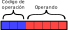
\includegraphics[height=4em]{img/instruccion.pdf}
        \end{figure}

\end{description}

\begin{tabularx}{\textwidth}{c|c|X}

    \textbf{Código de} & \textbf{Operando} &
    \multicolumn{1}{c}{\textbf{Descripción}} \\
    \textbf{operación} & & \\
    \emph{3 bits} & \emph{5 bits} & \\
    \hline
    \hline

    010 & \emph{dirección} & \textbf{Memoria → Acumulador}. Copia un byte
    desde la dirección de memoria al acumulador. \\
    \hline

    011 & \emph{dirección} & \textbf{Acumulador → Memoria}. Copia el contenido
    del acumulador en esa dirección de memoria. \\
    \hline

    100 & \emph{dirección} & \textbf{Suma}. El contenido de la dirección se
    suma al acumulador, y el resultado se almacena en el acumulador. \\
    \hline

    101 & \emph{dirección} & \textbf{Resta}. El contenido de la dirección se
    resta al acumulador, y el resultado se almacena en el acumulador. \\
    \hline

    110 & \emph{desplazamiento} & \textbf{Salto incondicional}. Se suma (en
    complemento a 2) el desplazamiento al \textbf{PC}. \\
    \hline

    111 & \emph{desplazamiento} & \textbf{Salto condicional}. Si el acumulador
    es cero, se suma (en complemento a 2) el desplazamiento al \textbf{PC}, en
    caso contrario el \textbf{PC} se incrementa en uno. \\
    \hline

    001 & \emph{(sin uso)} & \textbf{Detiene la maquina}. No se ejecutan
    nuevas instrucciones. Los registros y la memoria quedan con el último
    valor que tenían. \\
    \hline

    000 & \emph{(sin uso)} & \textbf{No operación}. No tiene ningún efecto
    sobre el acumulador ni memoria. El \textbf{PC} se incremente en uno. \\

\end{tabularx}



\end{document}
